\documentclass[a4paper]{scrreprt}
\usepackage{fullpage} % Slightly more margins
\usepackage{amsfonts}
\usepackage{fancyhdr}
\pagestyle{fancy}
\usepackage[english]{babel}
\selectlanguage{english}
\usepackage[utf8]{inputenc}
\usepackage{graphicx}
\usepackage{url}
\usepackage{textcomp}
\usepackage{amsmath}
\usepackage{lastpage}
\usepackage{pgf}
\usepackage{wrapfig}
\usepackage{fancyvrb}
\usepackage{listings} % Source code highlighting
\usepackage{algpseudocode} % Algorithms
\usepackage{courier}

% Create header and footer
\headheight 27pt
\pagestyle{fancyplain}
\lhead{\footnotesize{Object-Oriented Design, IV1350}}
\chead{}
\rhead{\footnotesize{Assignment 3 Report}}
\lfoot{}
\cfoot{\thepage (\pageref{LastPage})}

% Create title page
\title{Assignment 3}
\subtitle{Object-Oriented Design, IV1350}
\author{Emil Tullstedt emiltu@kth.se}
\date{2014-04-29}

\graphicspath{ {./images/} }
\lstset{basicstyle=\footnotesize\ttfamily, language=Java, numbers=left}

\begin{document}

\maketitle

\tableofcontents %Generates the TOC

\chapter{Introduction}
This report describes the implementation of a previously designed cache simulator made for a pregraduate project in the course \textbf{IV1350} at KTH in Stockholm. The implementation is not for production usage.

\begin{small}
While implementing the application, I co-operated with \textit{Martin Alge}, \textit{Jesper Falk} and \textit{Erik Pettersson}.
\end{small}

\chapter{Method}
In the process of procuring a working application that would run an implementation of the design bescribed in \textit{Assignment 2}\footnote{http://web.ict.kth.se/$\sim$emiltu/iv1350-emiltu-s2.pdf} Java were selected as being the preferred language in the documentation of the course.

The Java environment during the course of developing the application have consisted of the following:

\begin{itemize}
	\item OpenJDK Runtime Environment (\textbf{IcedTea} 2.4.4) (7u51-2.4.4-0ubuntu0.13.10.1)
	\item \textbf{rake} 10.3.0
	\item \textbf{rakejava} 1.3.7
	\item \textbf{javac} 1.7.0\_51
	\item \textbf{git} 1.8.3.2
\end{itemize}

As the application was already largely designed, implementation was made simplified. As the design was having a largely low coupling - it was possible to implement the separate classes for the design one by one, thus rapidly having a working application. The application were mostly written after the design with modifications were seemingly proper. During a period in the development process, the classes \texttt{CacheLayout} and \texttt{AddressLayout} was merged in the \texttt{CacheLayout}-class, but that idea was quickly scrapped since the class were dangerously close to becoming a megamodel containing most of the logic in the application.

The tests made their way into the application quite late, which have caused a couple of hours of unnecessary debugging for bugs that would've been quickly discovered if the tests had been written before the actual code of the application, as the bugs were mostly quite a proof of my errors.

\chapter{Result}
\label{sec:result}

\begin{figure}[h]
  \begin{center}
    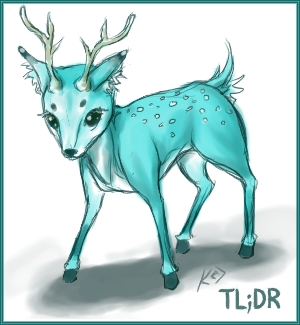
\includegraphics[scale=.5]{tldr.jpg}
    \caption{Teal Deer}
    \label{fig:sd}
  \end{center}
\end{figure}

\section{View, Controller and Startup}
\label{sec:sup}

In order to launch the application, there is need for a class handling the initialization of the controller and the view (which isn't fully covered in this report) and containing a \texttt{public static void main(String[] args)} function to be able to run the application from command-line. The class containing main is available in the \texttt{CacheSimulator}-class which source-code is available in subsection \ref{subsec:cachesimulator.java}.

The \texttt{CacheSimulator}-class initializes an object of the class \texttt{Controller} (which source is in subsection \ref{subsec:controller.java}) which handles the communication between the model classes and the \texttt{View}.


\subsection{Class: CacheSimulator}
\label{subsec:cachesimulator.java}

The \texttt{CacheSimulator} bootstraps the \texttt{Controller} (in \ref{subsec:controller.java}) and the \texttt{View} (in \ref{subsec:view.java})

\lstinputlisting[language=Java]{cachesim/source/is/mjuk/cache/CacheSimulator.java}

\subsection{Class: Controller}
\label{subsec:controller.java}

The \texttt{Controller} is responsible for the connection between the different models and any view.

\lstinputlisting[language=Java]{cachesim/source/is/mjuk/cache/Controller.java}

\subsection{Class: View}
\label{subsec:view.java}

The \texttt{View} simply keeps the application \texttt{Controller} (in \ref{subsec:controller.java}) connected to the user by presenting user friendly alternatives.

\lstinputlisting[language=Java]{cachesim/source/is/mjuk/cache/View.java}

\subsection{Class: Storage}
\label{subsec:storage.java}

The \texttt{Storage} is a non-persistent, singleton\footnote{i.e. there may ever only be a single \texttt{Storage}-object in existance in any one application.} storage unit, which keeps track of every single cache instruction (storing \texttt{InstructionDTO}s [which are referred to in \ref{subsec:instructiondto.java}]) and a couple of other data related to the application. The \texttt{Storage}-singleton may produce the vast majority of the content in a \texttt{SimulationDTO} (in \ref{subsec:simulationdto.java}) summarizing a single execution of the application. The \texttt{Storage}-object is written using TDD\footnote{The tests were written before the code} and it's tests are available at \ref{subsec:storagetest.java})

\lstinputlisting[language=Java]{cachesim/source/is/mjuk/cache/Storage.java}

\subsection{Class: SimulationDTO}
\label{subsec:simulationdto.java}

The \texttt{SimulationDTO} is a data transfer object that keeps track of a summarized essential data of a single run of a cache simulation.

\lstinputlisting[language=Java]{cachesim/source/is/mjuk/cache/SimulationDTO.java}

\section{User}
\label{sec:user}

The User-handling part of the application is the simplest, and is just taking care of a single string-object, the \textit{nickname} and a \textit{datetime}-stamp.

\subsection{Class: User}
\label{subsec:user.java}
\lstinputlisting[language=Java]{cachesim/source/is/mjuk/cache/User.java}

\section{Cache- and AddressLayout}
\label{sec:cache}

During the second phase of the application's runtime, the \texttt{Controller} (from subsection \ref{subsec:controller.java}) creates a \texttt{DataCache} (in \ref{subsec:datacache.java}) based on a user specified \texttt{CacheLayout} (in \ref{subsec:cachelayout.java}). It also associates an \texttt{AddressLayout} (in subsection \ref{subsec:addresslayout.java}) which can be used on the virtual cache contained within the \texttt{DataCache}.

The controller also stores the \texttt{CacheLayout} and \texttt{AddressLayout} data as a \texttt{LayoutDTO} (in \ref{subsec:layoutdto.java}) in the \texttt{Storage} singleton (from \ref{subsec:storage.java}) 

\subsection{Class: CacheLayout}
\label{subsec:cachelayout.java}

The \texttt{CacheLayout} is created by the controller with a \textit{BlockSize}, \textit{BlockCount} and \textit{Associativity}. The block size and the block count has to be powers of two while the associativity may be anything to your liking.

The \texttt{CacheLayout} creates a \texttt{AddressLayout} (in \ref{subsec:addresslayout.java}) by calculating it's properties from the \textit{BlockSize} and \textit{BlockCount} properties of the \texttt{CacheLayout}.
The following formulae is used to determine the size of the index and offset sizes of the \texttt{AddressLayout}

\begin{algorithmic}
\State $x \in \mathbb{R} \geq 0$ 
\If {$i \in 2^x$}
    \State $\text{size of address element} \gets \log _2 i$ 
\EndIf
\end{algorithmic}

Where \textit{i} is the \textit{BlockSize} in case of the offset and the \textit{BlockCount} for the index. In the case that either the block size or the block count isn't a power of two, the operation will fail with an IllegalArgumentException.

The final \texttt{AddressLayout} property is the tag size, which is $32 - (\text{indexSize} + \text{offsetSize})$ (assuming the 32-bit processor the simulator emulates).

\lstinputlisting[language=Java]{cachesim/source/is/mjuk/cache/CacheLayout.java}

\subsection{Class: AddressLayout}
\label{subsec:addresslayout.java}

The \texttt{AddressLayout} contains three objects, the \textit{tag size}, the \textit{index size} and the \textit{offset size}. These values are calculated from the \textit{BlockSize} and \textit{BlockCount} from the \texttt{CacheLayout} (in \ref{subsec:cachelayout.java}).

\lstinputlisting[language=Java]{cachesim/source/is/mjuk/cache/AddressLayout.java}

\subsection{Class: LayoutDTO}
\label{subsec:layoutdto.java}

The \texttt{LayoutDTO} is a data transfer object that contains data regarding the properties of \texttt{AddressLayout} (in \ref{subsec:addresslayout.java}) and the \texttt{CacheLayout} (in \ref{subsec:cachelayout.java}). It stores the block size, block count, associativity, tag size, index size and offset size of a single cache.

\lstinputlisting[language=Java]{cachesim/source/is/mjuk/cache/LayoutDTO.java}

\subsection{Class: AddressDTO}
\label{subsec:addressdto.java}

The \texttt{AddressDTO} is for transferring a parseable address. It is created by splitting an address to it's respective block size, block count and associativity fields.

\lstinputlisting[language=Java]{cachesim/source/is/mjuk/cache/AddressDTO.java}

\section{Instructions}

\subsection{Enum: InstructionType}
\label{subsec:instructiontype.java}
\lstinputlisting[language=Java]{cachesim/source/is/mjuk/cache/InstructionType.java}

\subsection{Class: Instruction}
\label{subsec:instruction.java}
\lstinputlisting[language=Java]{cachesim/source/is/mjuk/cache/Instruction.java}

\subsection{Class: InstructionDTO}
\label{subsec:instructiondto.java}
\lstinputlisting[language=Java]{cachesim/source/is/mjuk/cache/InstructionDTO.java}

\subsection{Class: DataCache}
\label{subsec:datacache.java}
\lstinputlisting[language=Java]{cachesim/source/is/mjuk/cache/DataCache.java}

\subsection{Class: Block}
\label{subsec:block.java}
\lstinputlisting[language=Java]{cachesim/source/is/mjuk/cache/Block.java}

\section{Tests}

\subsection{Class: CacheLayout Test}
\label{subsec:cachelayouttest.java}
\lstinputlisting[language=Java]{cachesim/test/is/mjuk/cache/CacheLayoutTest.java}

\subsection{Class: DataCache Test}
\label{subsec:datacachetest.java}
\lstinputlisting[language=Java]{cachesim/test/is/mjuk/cache/DataCacheTest.java}

\subsection{Class: Storage Test}
\label{subsec:storagetest.java}
\lstinputlisting[language=Java]{cachesim/test/is/mjuk/cache/StorageTest.java}

\section{Output from a run}
\lstinputlisting[language={}]{run.txt}

\chapter{Discussion}

\chapter{Attachements}

\subsection{Class: MisMath}
\label{subsec:mismath.java}
\lstinputlisting[language=Java]{cachesim/source/is/mjuk/utils/MisMath.java}

\end{document}
